\chapter{Stato dell'arte}

\section{Cloud Computing nell'era dei Big Data}

Il NIST (\textit{National Institute of Standards and Technology}) definisce il \textit{Cloud Computing} come un modello che promuove l'accesso globale alle risorse informatiche condivise, tipicamente \textit{on-demand} \cite{NISTCloudComputing}. L'infrastruttura di questo paradigma, nella sua versione più semplice, è relegata principalmente in \textit{data center}, ovvero dei raggruppamenti di risorse virtualizzate altamente accessibili che possono essere riconfigurate dinamicamente per garantire la scalabilità dei servizi. Questi fungono da nodi centrali e garantiscono agli utenti un'infrastruttura, una piattaforma oppure un servizio software utile per le loro applicazioni e i propri scopi (IaaS, Paas, SaaS).

Nonostante il \textit{Cloud Computing} abbia indubbiamente un ruolo chiave nel rendere accessibile una potenza di calcolo, altrimenti troppo difficile da poter essere realizzata in proprio, nella moderna era dei Big Data il tempo richiesto per accedere ad alcune applicazioni \textit{cloud-based}, che concentrano l'intera elaborazione dei dati nei suddetti \textit{data-center}, potrebbe essere troppo elevato e rendere questo paradigma impraticabile per applicazioni \textit{real-time} o, in generale, ovunque la latenza debba essere ridotta al minimo. Inoltre l'ormai noto incremento dei dispositivi connessi in ambito IoT (\textit{Internet of Things}) ed il relativo rapido aumento dei dati generati nell'\textit{edge} \footnote{Con \textit{edge} si intende la zona perimetrale della rete, in cui risiedono gli end-node. L'edge è caratterizzato da un punto di demarcazione (ad esempio un \textit{gateway}) che lo separa dal \textit{network core}, ovvero la parte centrale gestita dagli Internet Service Provider.} della rete richiedono che le risorse di calcolo siano geograficamente situate il più vicino possibile ai dispositivi stessi, così da diminuire al massimo la latenza, aumentando di conseguenza il \textit{throughput} della rete.

Per affrontare queste problematiche è quindi necessario garantire il cosiddetto \textit{Cloud-to-Thing Continuum}, ovvero la possibilità di rendere disponibili potenza computazionale, di storage e di networking ovunque nella rete, dal cloud agli end-nodes. In questo ambito sono state avanzate numerose proposte, ad esempio il \textit{Fog Computing}, sia in ambito industriale che accademico \cite{OpenFogReferenceArchitecture, FogComputingInIoT}.


\section{Fog Computing ed altri paradigmi nel Cloud-to-Thing Continuum}

\subsection{Fog Computing e architettura OpenFog}

Con \textit{Fog Computing} si intende un'architettura a livello di sistema che distribuisce le funzioni di elaborazione, archiviazione, controllo e rete più vicine agli utenti lungo un \textit{Cloud-to-Thing Continuum} \cite{OpenFogReferenceArchitecture}.

Il \textit{Fog Computing} dunque è innanzitutto caratterizzato da un approccio distribuito. Ciò deriva dal bisogno di superare i limiti dell'approccio centralizzato del Cloud Computing, come latenza, privacy e sovraccarico dei dati. In secondo luogo i nodi Fog, possono essere posizionati ovunque nella rete tra gli end-node e il cloud. Questa flessibilità che contraddistingue il Fog Computing, sottolinea la visione di questo paradigma non come una sostituzione, bensì come un'estensione del Cloud Computing, con lo scopo di colmare il divario tra quest'ultimo e i dispositivi IoT, garantendo quindi il continuum \textit{Cloud-to-Thing}.

Ad esempio, in un'applicazione che si occupa di analisi di Big Data prodotti da migliaia di dispositivi IoT, lo strato di Fog (dall'inglese Fog, \textit{Nebbia}) che si pone ad un livello "più basso", ovvero più vicino ai dispositivi, rispetto al Cloud (dall'inglese Cloud, \textit{Nuvola}) potrebbe svolgere una funzione di filtraggio, pre-elaborazione e aggregazione del flusso dati, rendendo eventualmente disponibili alcuni risultati ai livelli inferiori e alleggerendo il carico nel Cloud a cui rimarrebbero i task più complessi ma su una mole di dati molto ridotta e pre-elaborata.

\begin{figure}[!ht]
  \includegraphics[width=12cm]{images/FogCloudToThingContinuum}
  \centering
  \caption[Architettura OpenFog N-Tier]{Architettura OpenFog N-Tier \cite{OpenFogReferenceArchitecture}}
  \label{fig:ntier_architecture}
\end{figure}

Negli anni sono state proposte alcune architetture di particolare rilievo per scenari di Fog Computing. Molte ricerche fanno riferimento ad un'architettura a 3 livelli, composta da Cloud, Fog e IoT \cite{ThreeLevelArchitecture}. Per questo lavoro di Tesi l'architettura di riferimento è quella fornita dall'\textit{OpenFog Consortium}. Quest'ultimo è stato fondato da ARM, Cisco, Dell, Intel, Microsoft e dall'Università di Princeton, nel 2015. Ad oggi OpenFog e i suoi membri fanno parte dell'\textit{IIC} (\textit{Industrial Internet Consortium}). 

L'architettura di riferimento è detta \textit{N-Tier Architecture}, il cui schema è mostrato in Figura \ref{fig:ntier_architecture}. Questa mantiene comunque una struttura composta da tre macro-entità: il cloud, il livello Fog e gli end-node/dispositivi IoT. Il livello Fog, però, è ulteriormente scomposto in sotto-livelli (\textit{tier}) che più si allontanano dai dispositivi, più aumentano le loro capacità computazionali. Il numero di livelli Fog da adottare dipende dai requisiti dello scenario secondo diversi parametri, ad esempio il numero di dispositivi IoT, il carico di lavoro, le capacità dei nodi ad ogni livello, i requisiti di latenza minima e così via. Inoltre i nodi Fog in ogni tier possono essere collegati tra loro formando una maglia capace di fornire caratteristiche aggiuntive, come resilienza, tolleranza ai guasti, bilanciamento del carico e così via. Questo significa che i nodi sono in grado di comunicare sia orizzontalmente che verticalmente all'interno dell'architettura Fog.

I vantaggi fondamentali dell'architettura di riferimento definita dall'OpenFog Consortium sono riassunti con il termine \textit{SCALE} \cite{OpenFogReferenceArchitecture}, ovvero:

\begin{itemize}
	\item \textbf{Security}. Sicurezza aggiuntiva per garantire transazioni sicure e affidabili. Dal \textit{Security Pillar} dell'architettura di riferimento, si evince la necessità di uno o più "nodi fidati" (\textit{Root of Trust}) quando si trattano dati sensibili.
	\item \textbf{Cognition}. L'infrastruttura Fog è consapevole dei requisiti e degli obiettivi delle applicazioni, quindi distribuisce le capacità di elaborazione, comunicazione, controllo e archiviazione lungo il continuum Cloud-to-Things, creando applicazioni che soddisfano meglio le esigenze specifiche dello scenario.
	\item \textbf{Agility}. Lo sviluppo di un nuovo servizio è solitamente lento e costoso, a causa dei costi e dei tempi necessari ai grandi fornitori per avviare o adottare l'innovazione. Il Fog Computing, invece, offre innovazione rapida e scalabilità conveniente, in cui individui e piccoli team possono utilizzare strumenti di sviluppo aperti (ad esempio API e SDK, secondo il pilastro \textit{Openness} definito da OpenFog \cite{OpenFogReferenceArchitecture}) e la proliferazione di dispositivi IoT per offrire nuovi servizi.
	\item \textbf{Latency}. L'architettura Fog supporta l'elaborazione e l'archiviazione dei dati vicino all'utente, con conseguente bassa latenza. Pertanto, il Fog computing soddisfa perfettamente la richiesta di elaborazione in tempo reale, in particolare quindi per le applicazioni \textit{real-time}.
	\item \textbf{Efficiency}. Riconoscimento e condivisione delle risorse inutilizzate dei dispositivi finali che partecipano al networking.
\end{itemize}

\subsection{Possibili applicazioni del Fog Computing}

\subsubsection{Smart Cars e Traffic Control}

I veicoli smart (\textit{Smart Cars}) sono in grado di produrre giornalmente svariati terabyte di dati grazie alla combinazione di sensori \textit{LIDAR} \footnote{LIDAR (\textit{Light Detection and Ranging}) è un metodo per determinare la presenza di oggetti, la loro forma e la loro distanza dall'osservatore utilizzando un laser e misurando il tempo necessario alla luce riflessa per tornare al trasmettitore laser.}, dei sensori GPS, delle videocamere intelligenti a bordo dei veicoli per il riconoscimento delle immagini e così via. Oltre ai dati prodotti dalle \textit{Smart Cars} ci sono quelli generati dai sistemi di controllo intelligenti, ovvero l'infrastruttura del \textit{Traffic Control} (semafori intelligenti, sensori di rilevamento del traffico e delle congestioni, videocamere, ecc.). È evidente come un modello \textit{cloud-only} non sia adatto, vista l'enorme mole di dati, a garantire un throughput sufficientemente elevato. Un'architettura Fog potrebbe invece soddisfare le particolari esigenze di questo scenario. In quest'ultimo, i veicoli sono nodi Fog che comunicano tra loro, o con i sistemi di controllo. In particolare i nodi Fog a bordo delle \textit{Smart Cars} possono offrire i normali servizi di \textit{infotainment}, ADAS \footnote{ADAS (\textit{Advanced Driver Assistance Systems}) è un insieme di tecnologie che assistono il guidatore nelle operazioni di guida e parcheggio in modo sicuro.}, guida autonoma, sistemi anticollisione, navigazione, e così via, tramite la connessione all'infrastruttura Fog con l'ausilio di diverse tecnologie, come DSRC (\textit{Dedicated Short Range Communications}) o le reti cellulari (3G, LTE, 5G, etc.).

\begin{figure}[!ht]
  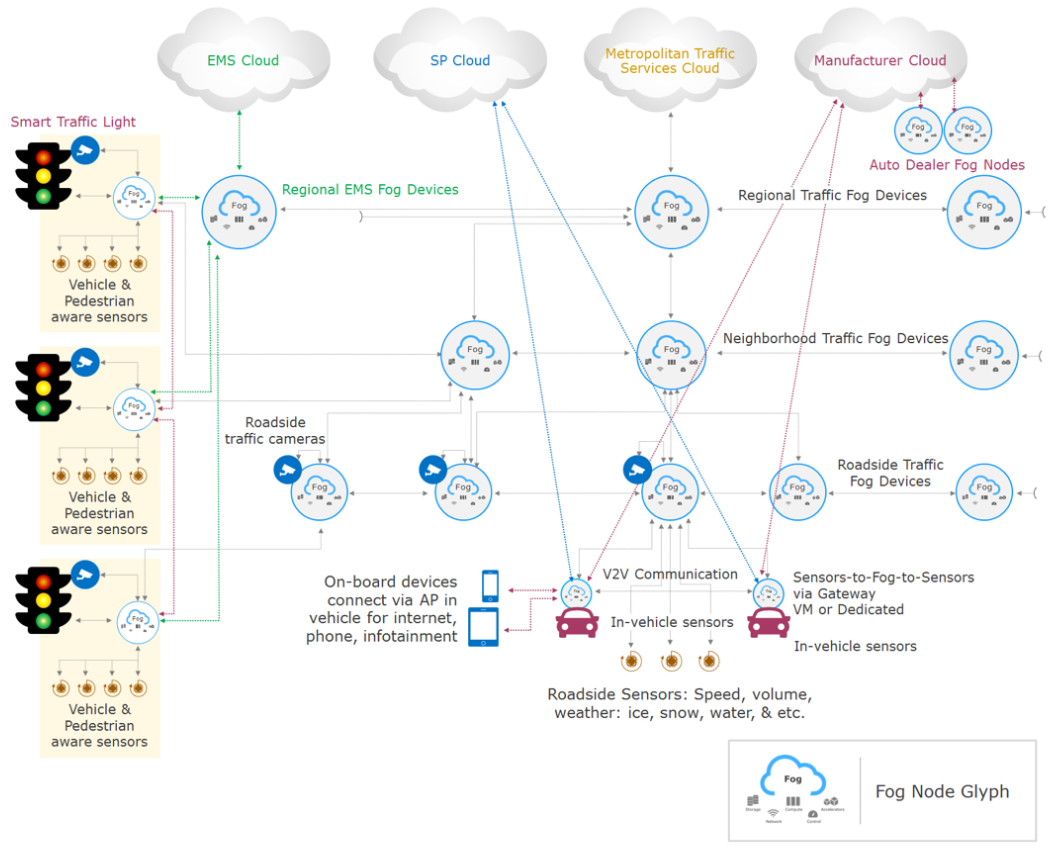
\includegraphics[width=14cm]{images/smartcars_trafficcontrol}
  \centering
  \caption[Architettura di uno scenario Fog in ambito Smart Cars e Traffic Control]{Architettura di uno scenario Fog in ambito Smart Cars e Traffic Control \cite{OpenFogReferenceArchitecture}}
  \label{fig:smartcars_trafficcontrol}
\end{figure}

L'architettura di riferimento, mostrata in Figura \ref{fig:smartcars_trafficcontrol}, è strutturalmente gerarchica, con 3 livelli di nodi Fog. Il primo livello (\textit{Roadside Fog Nodes}) si occupa di raccogliere i dati dai vari sensori e telecamere. I nodi Fog in questo livello eseguono alcune veloci analisi, utili ad esempio a comunicare ai veicoli in transito particolari condizioni del traffico o della strada. I dati aggregati dal primo livello sono inviati al secondo e/o al terzo livello (non c'è necessariamente una gerarchia nelle comunicazioni, questo per definizione dell'architettura Fog e della sua flessibilità), ovvero i \textit{Neighborhood Fog Nodes} e i \textit{Regional Fog Nodes}. In genere, ogni livello Fog nella gerarchia fornirà ulteriori capacità di elaborazione, storage e rete. Ad esempio, livelli di gerarchicamente più alti garantiranno un trattamento aggiuntivo per fornire analisi dei dati o capacità di archiviazione di grandi dimensioni, utili ad esempio per analisi sul lungo periodo o per inviare dati ad altre zone della rete stradale per particolari task.

\subsubsection{Smart Cities e Smart Buildings}

Un altro interessante impiego del Fog Computing è nell'ambito delle \textit{Smart Cities} e degli \textit{Smart Buildings}. Infatti sebbene  la maggior parte delle città moderne disponga di una o più reti cellulari che forniscono una copertura dell'intera città, queste reti hanno spesso limiti di capacità e larghezza di banda che soddisfano appena le esigenze degli attuali abbonati. Ciò lascia poca larghezza di banda per i servizi più avanzati previsti in una città intelligente nell'era dei Big Data, come \textit{Smart Parking}, \textit{Traffic Control}, ospedali intelligenti, controllo sul consumo elettrico e così via.  

\begin{figure}[!ht]
  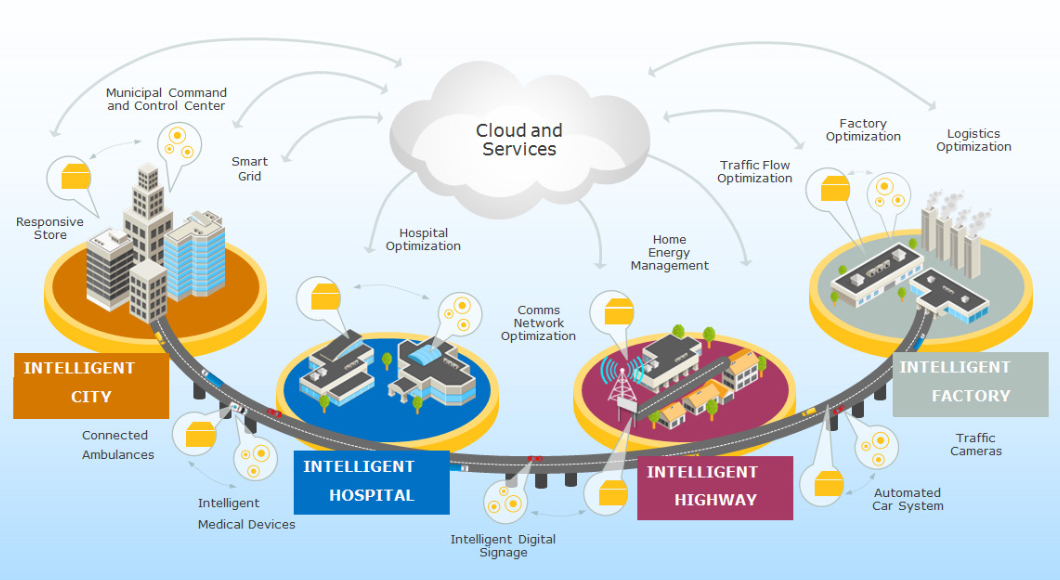
\includegraphics[width=14cm]{images/smartcities_smartbuildings}
  \centering
  \caption[Opportunità per una Smart City]{Opportunità per una \textit{Smart City} \cite{OpenFogReferenceArchitecture}}
  \label{fig:smartcars_trafficcontrol}
\end{figure}


Questo caso d'uso è già realtà, ad esempio, nella città di Barcellona, dove i risultati hanno dimostrato che il Fog Computing è la possibile chiave di volta per l'implementazione di servizi molto avanzati e complessi, in città che producono decine di milioni di Gigabyte di dati giornalmente \cite{FogBarcellona}. 

\subsection{Altri Paradigmi}

Per analizzare i vari altri paradigmi che possono essere considerati un'estensione, più che un'alternativa al Fog Computing, è utile introdurre il concetto di \textit{Edge Computing}. Quest'ultimo è un un paradigma nato dall'esigenza di spostare la capacità di calcolo verso l'edge \footnote{Con \textit{edge} si intende la zona perimetrale della rete, in cui risiedono gli end-node. L'edge è caratterizzato da un punto di demarcazione (ad esempio un \textit{gateway}) che lo separa dal \textit{network core}, ovvero la parte centrale gestita dagli Internet Service Provider.} della rete. In \cite{EdgeComputing} viene definito l'Edge Computing come \textit{"tecnologie abilitanti che consentono di effettuare calcoli ai margini della rete sui dati, a valle per conto di servizi cloud e a monte per conto di servizi IoT"}. L'idea è quella di estendere le capacità dal cloud all'edge della rete, con l'obiettivo di portare la potenza di calcolo il più vicino possibile ai generatori dei dati, ovvero ai dispositivi IoT. Nonostante sia il Fog Computing che l'Edge Computing muovano le capacità computazionali vicino agli end-node, OpenFog afferma che l'Edge Computing venga erroneamente chiamato Fog Computing (e viceversa): la fondamentale distinzione sta nel fatto che il Fog Computing è strutturalmente gerarchico e fornisce potenza computazionale, networking e storage ovunque nella rete, dal Cloud agli end-node (\textit{Cloud-to-Thing Continuum}), mentre l'Edge Computing tende ad essere limitato all'edge \cite{OpenFogReferenceArchitecture}.

I principi fondanti dell'Edge Computing possono essere messi in pratica in diversi modi, in termini di tipo di dispositivi utilizzati, protocolli di comunicazione adottati e così via. I principali paradigmi sono esposti nel seguito.

\subsubsection{Mobile Cloud Computing e Cloudlet Computing}

Il \textit{Mobile Cloud Computing} (MCC) è basato sul concetto del \textit{mobile offloading}: l'idea alla base, per un dispositivo mobile, è quella di delegare, quando possibile, storage e calcoli ad entità remote (ad esempio il cloud) in modo da ridurre il carico di lavoro e ottimizzare il consumo di energia. In realtà oggi il concetto di MCC è stato esteso tenendo in considerazione i principi dell'Edge Computing. La nuova interpretazione del MCC è quella di delegare l'elaborazione e lo storage dei dati a dispositivi situati all'edge della rete, piuttosto che al cloud. L'implementazione più comune di questa visione è il \textit{Cloudlet Computing} (CC), che consiste nell'utilizzare dei \textit{cloudlet} \footnote{Un \textit{cloudlet} è una piccola infrastruttura cloud \textit{affidabile}, situata nell'edge della rete disponibile per i dispostivi mobili vicini, che collabora con il cloud per servire i dati in modo più efficiente.} per eseguire elaborazione ed archiviazione dei dati vicino ai dispositivi finali.

\subsubsection{Multi-access Edge Computing}

Esattamente come il \textit{Mobile Cloud Computing} è un'estensione del \textit{Mobile Computing} attraverso il \textit{Cloud Computing}, analogamente, il \textit{Multi-access Edge Computing} (MEC) è un'estensione del \textit{Mobile Computing} attraverso l'\textit{Edge Computing}. In \cite{MultiAccessEdgeComputing} il MEC viene definito come una piattaforma che fornisce funzionalità IT e di cloud computing all'interno della \textit{Radio Access Network} (RAN) in 4G e 5G, in prossimità dei dispositivi mobili. Il Multi-access Edge Computing è stato precedentemente definito come \textit{"Mobile Edge Computing"}, ma il paradigma è stato ampliato per includere una più ampia gamma di applicazioni oltre alle attività specifiche per dispositivi mobili. Esempi di applicazioni di MEC includono analisi video, \textit{Smart Cars}, monitoraggio della salute e realtà aumentata.

%Un paradigma architetturale di notevole importanza è l'\textit{Edge Computing}. La sua caratteristica principe è quella di spostare la potenza computazionale all'edge della rete. Nonostante sia il Fog Computing che l'Edge Computing muovano le capacità computazionali vicino agli end-node, OpenFog afferma che l'Edge Computing venga erronaemente chiamato Fog Computing (e viceversa): la fondamentale distinzione sta nel fatto che il Fog Computing è strutturalmente gerarchico e fornisce potenza computazionale, networking e storage ovunque nella rete, dal Cloud agli end-nodes (\textit{Cloud-to-Thing Continuum}), mentre l'Edge Computing tende ad essere limitato all'edge \cite{OpenFogReferenceArchitecture}.

%L'avanzamento di tecnologie come il Fog Computing può essere stato facilitato dagli sviluppi del \textit{Mobile Computing}. Con Mobile Computing si intende quella situazione in cui l'elaborazione dei dati avviene sui dispositivi mobili e portatili, come laptop, tablet o smartphone. Il suo punto cardine è l'adattamento in un qualsiasi ambiente con una potenza computazionale e connettività di rete scarsa o intermittente. Ci sono diversi problemi però che impediscono al Mobile Computing di soddisfare le attuali esigenze nell'era dei Big Data come ad esempio la troppo poca potenza computazionale, lo scarso bilanciamento tra autonomia e dipendenza da altri dispositivi, latenza nella comunicazione e così via. Nonostante queste problematiche, alcune soluzioni possono prevedere un'integrazione con il Cloud, come indicato dal NIST, per permettere l'implementazione di applicazioni CPU e data-intensive \cite{NISTMobileCloudComputing}. 

\subsubsection{Mist Computing}

Spesso chiamato anche \textit{IoT Computing}, il \textit{Mist Computing} viene impiegato per raggiungere l'edge più estremo dei dispositivi connessi (micro-controllori e sensori) \cite{MistComputing}. Il Mist Computing può essere visto come la prima posizione di calcolo nel continuum IoT-Fog-Cloud. Infatti può aiutare a conservare la larghezza di banda e la carica della batteria poiché sono solo i dati essenziali ad essere trasmessi al gateway, al server o al router. Inoltre il Mist Computing offre l'utilizzo di meccanismi di controllo dell'accesso ai dati che possono garantirne la riservatezza a livello locale. Di contro, questo paradigma ha che i micro-controllori e i sensori utilizzati nell'infrastruttura possono essere utilizzati solo per un'elaborazione leggera, pertanto il loro utilizzo è ristretto ad un numero piuttosto esiguo di applicazioni, a meno dell'implementazione dello stesso nel continuum Clout-to-Thing venendo quindi incluso in un'architettura più ampia, basata ad esempio sul Fog Computing \cite{MistComputingFutureDirections}.

\section{Simulatori di Fog Computing}

La progettazione e l'ottimizzazione di sistemi distribuiti su larga scala, richiedono una descrizione realistica del flusso dei dati, della mole enorme di richieste emesse dai nodi, dei servizi disponibili e ogni aspetto necessario alla comprensione del comportamento di sistemi che scambiano dosi massicce di dati. La via più semplice per comprendere le potenzialità e allo stesso tempo i limiti di scenari così complessi è quella della \textit{simulazione}.

La ricerca nell'ambito del Fog Computing vanta un numero consistente di strumenti di simulazione più o meno avanzati. Tra i più noti vi sono \textit{iFogSim} \footnote{Disponibile su: \url{https://github.com/cloudslab/ifogsim}} \cite{iFogSim} ed \textit{EdgeCloudSim} \footnote{Disponibile su: \url{https://github.com/CagataySonmez/EdgeCloudSim}} \cite{EdgeCloudSim}, entrambi basati su \textit{CloudSim}, un simulatore di architetture cloud. Oltre alla simulazione un altro importate strumento che garantisce esperimenti ripetibili e controllabili è l'\textit{emulazione}. Tra i software più rilevanti esistono \textit{EmuFog} \footnote{Disponibile su: \url{https://github.com/emufog/emufog}} \cite{EmuFog} e \textit{FogBed} \footnote{Disponibile su: \url{https://github.com/fogbed/fogbed}} \cite{FogBed}. Entrambi consentono all'utente di progettare scenari Fog con applicazioni basati su Docker o Mininet.

\subsection{YAFS, \textit{Yet Another Fog Simulator}}

Per questo lavoro di tesi, è stato utilizzato, tra le altre cose, il simulatore \textit{YAFS} \footnote{Disponibile su: \url{https://github.com/acsicuib/YAFS}} (\textit{Yet Another Fog Simulator}), un simulatore ad eventi discreti sviluppato in Python e basato su \textit{SimPy}, ovvero un framework DES (\textit{Discrete Event Simulator}) basato sui processi anch'esso sviluppato in Python \cite{YAFSSimulator}. YAFS è progettato per analizzare progettare applicazioni in scenari Fog e incorpora le strategie per il placement, lo scheduling e l'instradamento dei dati. I punti chiave che hanno portato alla scelta di YAFS sono esposti nel seguito:
\begin{itemize}
	\item \textbf{Placement, Scheduling, Routing e processi personalizzati}. L'algoritmo di placement viene invocato all'avvio e viene eseguito durante la simulazione secondo una distribuzione personalizzata. L'algoritmo di routing sceglie il percorso che collega il trasmettitore e il recettore e l'algoritmo di scheduling sceglie l'applicazione che deve eseguire il task associato alla richiesta. Oltre agli algoritmi appena esposti che possono essere definiti dall'utente, quest'ultimo può implementare funzioni personalizzate che possono essere invocate in fase di esecuzione per fornire implementazioni flessibili di eventi reali come il movimento delle fonti del carico di lavoro, la generazione di guasti della rete e la raccolta di dati specifici utilizzando anche applicazioni di terze parti.
	\item \textbf{Creazione dinamica delle sorgenti dei messaggi}. Ogni fonte di carico di lavoro rappresenta la connessione alla rete di un utente, di un sensore IoT o di un attuatore che richiede un servizio. Ogni sorgente è associata ad un'entità DES di rete che genera richieste secondo una distribuzione personalizzata. Le sorgenti del carico di lavoro possono essere create, modificate o rimosse dinamicamente, consentendo la modellazione dei movimenti degli utenti in un generico ecosistema.
	\item \textbf{Topologia della rete}. YAFS basa la struttura della topologia sulla \textit{Complex Network Theory}, grazie all'implementazione della libreria \textit{NetworkX}, da cui deriva la possibilità di applicare tutti gli algoritmi che ne derivano, ottenendo quindi indicatori di maggior interesse sulle topologie adottate.
	\item \textbf{Risultati}. YAFS esegue la registrazione automatica basata su CSV di due tipi di eventi: 
	\begin{itemize}
		\item generazione del carico di lavoro e del calcolo eseguito su di esso
		\item trasmissioni dei messaggi sui collegamenti. 
	\end{itemize}
	
	I risultati sono salvati in formato \textit{raw} con un impronta noSql con l'idea che da dati in formati più semplici derivino analisi più veloci.
\end{itemize}












